\section{Design}

\subsection{AI Criteria}

\label{criteria}
The overall process that was found when performing an epic breakdown is a combination of clustering related requirements, specifications, and details along with the further breakdown of complex info into smaller stories and tasks. Clustering can be performed in either supervised or unsupervised learning. Supervised learning requires the existence of a data set that has been correctly labeled. Although a general data set of decomposed epics can be generated, it was deemed that the range of topics an epic can encompass was too large to have a trained model that would accurately cluster the content of an epic. 

Additionally, an early assumption made about the decomposition process is that the text processing techniques should not rely upon the existence of historical project information, whether that be in the form of previously completed epics or sprints. As a result, unsupervised clustering techniques were only considered as they allowed for the decomposition process to be applicable to new projects, which lack history, and projects that have not been topically available to train a clustering model off of.

The last criteria for the text processing approaches under consideration was that no additional information should be generated through AI. This was due to the previously discussed lack of data, specific to the project domain, that could be used to potentially generate stories and tasks.

\begin{table}
\begin{tabularx}{\textwidth}{|c|c|c|c|}
\hline
Component & Options & Choice & Reasoning \\
\hline
Epic Decomposition & 
\begin{itemize}
\item KMeans
\item Meanshift
\item DBSCAN
\item OPTICS
\end{itemize} &
Mean-shift & All of the mentioned clustering algorithms are dynamic as they do not require the number of clusters as input. Mean-shift only requires the size of the region to search through (bandwidth), which can be estimated, where all other options require arbitrary values to create clusters.\\
\hline
\end{tabularx}
\end{table}

\subsection{Epic Decomposition}


\subsection{Story Optimization}


\subsection{Task Generation}

Task generation was identified as the process of breaking down a requirement into its most simplest form. Based on the criteria laid out in \nameref{criteria}, simplification on the existing input of requirements could be completed by deconstructing complex sentences into simple sentences. 

The first process to break down sentences was to use parts-of-speech tagging to remove any unnecessary words from the sentence; this was done by identifying stopwords, since simple sentences contain only one subject and predicate. Therefore, using the word dependency we were able to determine which words were connected to the subject. By making sure the sentence contained one subject and verb we were able to create a complete simple sentence. Everytime a new subject was found that meant a new sentence was needed. Each simple sentence generated from the stories can then be suggested as tasks.

\subsection{Flow}

\begin{figure*}
\centerline{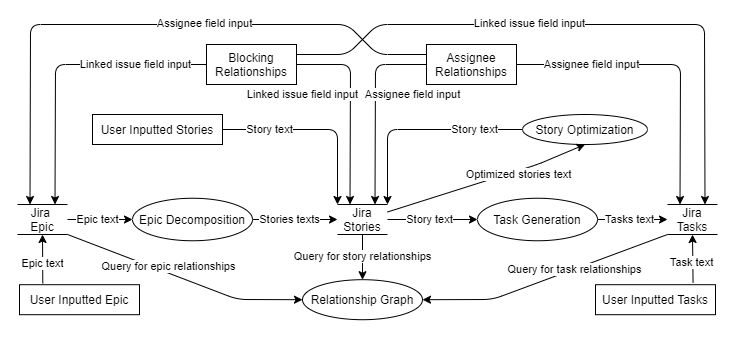
\includegraphics[width=\textwidth,height=\textheight,keepaspectratio]{./figure/DataflowDiagram.png}}
\caption{Data Flow diagram showing the various entry points, sources of data, and processes within Jira and AI4Agile}
\end{figure*}

\begin{figure*}
\centerline{\includegraphics[width=\textwidth,height=\textheight,keepaspectratio]{./figure/ExampleDataFlowDiagram.png}}
\caption{Simplified Data Flow diagram outlining the flow of the decomposition processes}
\end{figure*}


\subsection{Relationship visualization}